\newpage
\thispagestyle{empty}
% OBS: Coloque sempre o que você quer deixar de fundo na página como primeiro comando

% Imagem de fundo - crie um arquivo separado em tamanho A4 (210x297mm) no formato pdf
\begin{tikzpicture}[remember picture,overlay]
    % Inclui a imagem em segundo plano
    \node[anchor=center,inner sep=0pt] at (current page.center) {
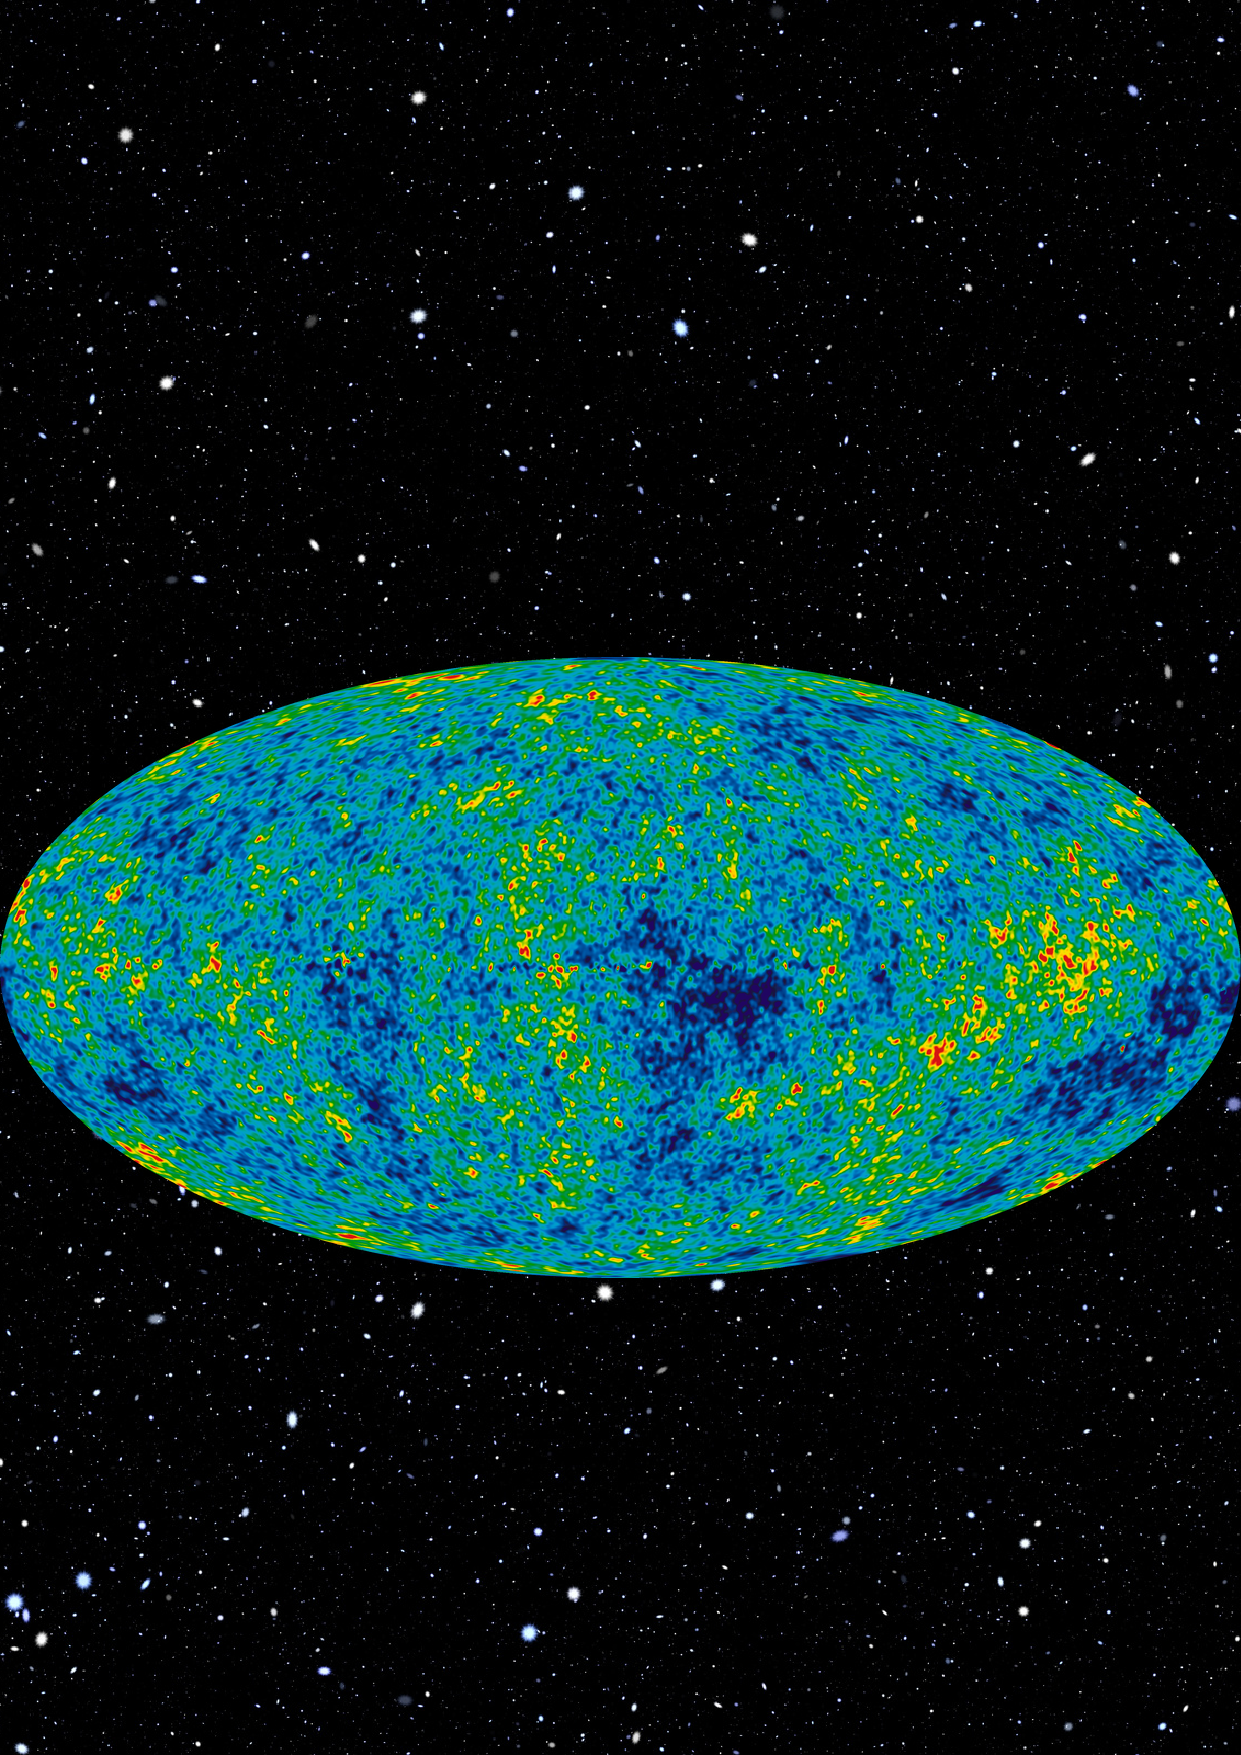
\includegraphics[width=\paperwidth,height=\paperheight,keepaspectratio]{Capa/Figuras_Capa/WMAP_Capa.pdf}
    };
\end{tikzpicture}

% Desenha um retângulo (branca)
\begin{tikzpicture}[remember picture, overlay]
    \draw[line width=7.4cm, white] 
        ($(current page.west) + (0,10.4)$) -- ($(current page.east) + (0,10.4)$);
\end{tikzpicture}

% Desenha um retângulo (cor da edição)
\begin{tikzpicture}[remember picture, overlay]
    \draw[line width=7cm, base] 
        ($(current page.west) + (0,10.4)$) -- ($(current page.east) + (0,10.4)$);
\end{tikzpicture}

% Nome da revista
\vspace{-3.2cm} % Ajuste a distância vertical para que o nome da revista fique centralizado com a linha horizontal
\begin{center}
    {\norwester\myfontsizeNewstonCapa NEWSTON}
\end{center}
\begin{center}
    {\bebasneue\myfontsizeJornalCapa \textls[530]{JORNAL}}
\end{center}

% Ajuste os valores em \textls[] (espaço entre letras) e na coordenada y de \node para adequar o tema e número com data da edição dentro do retângulo
\begin{tikzpicture}[remember picture, overlay]
    \node[anchor=north] at ($(current page.north west) + (0.5cm,-1.15cm)$) {
        \rotatebox{90}{\bebasneuebold\myfontsizeTemaCapaVerticalECC \textls[280]{HISTÒRIA\, DO\, UNIVERSO}}
    };
\end{tikzpicture}

\begin{tikzpicture}[remember picture, overlay]
    \node[anchor=north] at ($(current page.north west) + (20.5cm,-1.3cm)$) {
        \rotatebox{90}{{\bebasneuebold\myfontsizeTemaCapaVerticalECC \textls[200]{EDIÇÃO \NumeroEdicao -}} {\bebasneue\myfontsizeTemaCapaVerticalECC\textls[200]{\MakeUppercase{\DataEdicao}}}}
    };
\end{tikzpicture}

% Tema da edição
\hspace{-1.5cm}{\cooperheavy\myfontsizeTema\echoShadowText{baseechoshadow}{baseshadow}{História do Universo:}}

% Logo da UEM Branco
\begin{tikzpicture}[remember picture, overlay]
    % Ajuste a posição da figura conforme necessário
    \node[anchor=south, yshift=19cm, xshift=8cm] at (current page.south) { % Deslocamento vertical e horizontal na página - altere de acordo com o local em que deseja posicionar a logo
        
\includegraphics[width=0.23\textwidth]{Figuras_Capa_ContraCapa/UEM_Logo_Modelo_Branco.png}
    };
\end{tikzpicture}

% Desenha um retângulo (branca)
\begin{tikzpicture}[remember picture, overlay]
    \draw[line width=1.9cm, white] 
        ($(current page.west) + (0,-12.8)$) -- ($(current page.east) + (0,-12.8)$);
\end{tikzpicture}

% Desenha um retângulo (cor da edição) que engloba um título de artigo (diminua ou aumente a coordenada em x do segundo conjunto de coordenadas)
\begin{tikzpicture}[remember picture, overlay]
    \draw[line width=1.7cm, base] 
        ($(current page.west) + (0.1,-12.8)$) -- ($(current page.east) + (-12,-12.8)$);
\end{tikzpicture}

% Títulos de Artigos na Capa com TikZ (altere as coordenadas para posicionar o título do artigo dentro do retângulo de sua preferência)
\begin{tikzpicture}[remember picture, overlay]
    \node[anchor=north west, inner sep=0pt, outer sep=0pt] at ($(current page.north west) + (0.5cm,-27.2cm)$) {
        {\cooperbold\myfontsizeTitulosArtigosCapa Á Luz de Caravaggio}
    };
\end{tikzpicture}

% Desenha um retângulo (cor da edição) que engloba um título de artigo (diminua ou aumente a coordenada em x do primeiro e segundo conjunto de coordenadas)
\begin{tikzpicture}[remember picture, overlay]
    \draw[line width=1.7cm, base] 
        ($(current page.west) + (9.1,-12.8)$) -- ($(current page.east) + (-6.5,-12.8)$);
\end{tikzpicture}

% Títulos de Artigos na Capa com TikZ (altere as coordenadas para posicionar o título do artigo dentro do retângulo de sua preferência) para textos em duas linhas use \myfontsizeTitulosArtigosCapaDois para diminuir o tamanho da fonte
\begin{tikzpicture}[remember picture, overlay]
    \node[anchor=north west, inner sep=0pt, outer sep=0pt, text width=10cm] at ($(current page.north west) + (10cm,-27cm)$) {
        {\cooperbold\myfontsizeTitulosArtigosCapaDois Tipos de \\ Radiações}
    };
\end{tikzpicture}

\begin{tikzpicture}[remember picture, overlay]
    \draw[line width=1.7cm, base] 
        ($(current page.west) + (14.6,-12.8)$) -- ($(current page.east) + (-0.1,-12.8)$);
\end{tikzpicture}

\begin{tikzpicture}[remember picture, overlay]
    \node[anchor=north west, inner sep=0pt, outer sep=0pt, text width=10cm] at ($(current page.north west) + (15.5cm,-27cm)$) {
        {\cooperbold\myfontsizeTitulosArtigosCapaDois A Física dos\\ Esportes}
    };
\end{tikzpicture}


%{\cooperheavy\myfontsizeTituloTema ERA\\PRIMORDIAL}

%\begin{tikzpicture}[remember picture, overlay]
    %\node[anchor=center, inner sep=0pt, outer sep=0pt] at ([shift={(-1.5cm,-8.5cm)}] current page.center) {
      %  \begin{tikzpicture}
         % Múltiplos nós para criar um efeito de sombra esmaecida
        %    \foreach \angle in {0, 30, 60, 90, 120, 150, 180, 210, 240, 270, 300, 330} {
              %  \node[anchor=center, inner sep=0pt, outer sep=0pt, opacity=0.1, text=purple] at (\angle:0.2cm) {
               %     {\cooperheavy\myfontsizeTituloTema \shortstack[l]{ERA\\[0.5ex] PRIMORDIAL}}
              %  };
           % }
            % Texto principal
           % \node[anchor=center, inner sep=0pt, outer sep=0pt] {
             %   {\cooperheavy\myfontsizeTituloTema \shortstack[l]{ERA\\[0.5ex] PRIMORDIAL}}
          %  };
       % \end{tikzpicture}
  %  };
%\end{tikzpicture}

%\textcolor[gray]{\textopacity{0.5}{Este é um exemplo de texto esmaecido com opacidade de 50\%.}}


\begin{tikzpicture}[remember picture, overlay]
    \node[anchor=center, inner sep=0pt, outer sep=0pt] at ([shift={(-1.5cm,-8.5cm)}] current page.center) {
        \begin{tikzpicture}
             % Texto principal com contorno
            \node[anchor=center, inner sep=0pt, outer sep=0pt] {
                {\cooperheavy\myfontsizeTituloTema \contour{base}{\shortstack[l]{ERA\\[0.5ex] PRIMORDIAL}}}
            };
        \end{tikzpicture}
    };
\end{tikzpicture}


